\tikzstyle{every node}=[thick,anchor=west, rounded corners, font={\scriptsize\ttfamily}, inner sep=2.5pt]
\tikzstyle{selected}=[draw=black,fill=black!10]
\tikzstyle{root}=[selected, fill=black!20]

\addchap{GCW Widgets}
\section{Structuring the layout}
\subsection{GCWDivider}
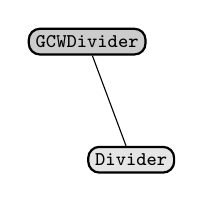
\begin{tikzpicture}
    \node [root] {GCWDivider}
    child { node [selected] {Divider}
    };
\end{tikzpicture}
\captionof{figure}{GCWDivider}
\label{fig: GCWDivider}
\begin{table}[H]
\begin{tabular}[h]{p{2cm}p{9cm}}
    \caption{GCWDivider}
    Aim       & Draws a horizontal line\\
    Import    & GCWizard/lib/widgets/common/base/gcw\_divider.dart\\
    Parameter & --\\
    \label{tab:GCWDivider}
\end{tabular}
\end{table}
\paragraph*{Example} \,
\begin{figure}[H]
    \centering
    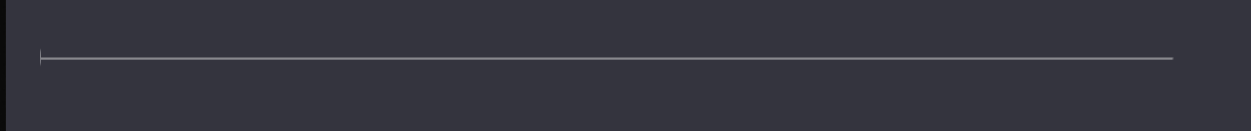
\includegraphics[height=0.75cm]{Bilder/Divider}
    \caption[]{Example GCWDivider}
    \label{fig:GCWDivider}
\end{figure}
\begin{lstlisting}
Widget build(BuildContext context) {
    return Column(
        children: <Widget>[
            ...
            GCWDivider(),
            ...
        ],
    );
}
\end{lstlisting}
\captionof{lstlisting}{Example GCWDivider}
\label{fig: ExampleGCWDivider}

\newpage
\subsection{GCWTextDivider}
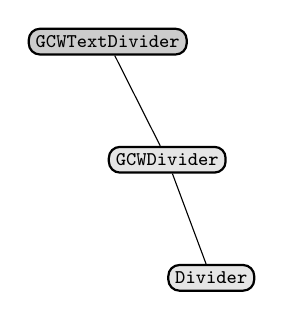
\begin{tikzpicture}
    \node [root] {GCWTextDivider}
    child { node [selected] {GCWDivider}
        edge from parent [-]
        child { node [selected] {Divider}
        };
    };
\end{tikzpicture}
\captionof{figure}{GCWTextDivider}
\label{fig: GCWTextDivider}
\begin{table}[H]
\begin{tabular}[h]{p{2cm}p{9cm}}
    \caption{GCWTextDivider}
    Aim       & Prints a text and fill with a horizontal line.\\
    Import    & GCWizard/lib/widgets/common/gcw\_text\_divider.dart\\
    Parameter & text String\\
    \label{tab:GCWTextDivider}
\end{tabular}
\end{table}
\paragraph*{Example} \,
\begin{figure}[H]
    \centering
    
\includegraphics[height=0.75cm]{Bilder/TextDivider}
    \caption[]{Example GCWTextDivider}
    \label{fig:GCWTextDivider}
\end{figure}
\begin{lstlisting}
Widget build(BuildContext context) {
    return Column(
        children: <Widget>[
            ...
            GCWTextDivider(
                text: i18n(context, 'common_output')
            ),
            ...
        ],
    );
}
\end{lstlisting}
\captionof{lstlisting}{Example GCWTextDivider}
\label{fig: ExampleGCWTextDivider}

\newpage
\section{Input}
\subsection{GCWTextfield}
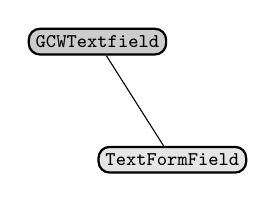
\begin{tikzpicture}
    \node [root] {GCWTextfield}
    child { node [selected] {TextFormField}
        edge from parent [-]
    };
\end{tikzpicture}
\captionof{figure}{GCWTextfield}
\label{fig: GCWTextfield}
\begin{table}[H]
\begin{tabular}[h]{p{2cm}p{9cm}}
    \caption{GCWTextfield}
    Aim       & Get an input; with a given TextInputFormatter you can mask the input\\
    Import    & GCWizard/lib/widgets/common/base/gcw\_textfield.dart\\
    Parameter & TextEditingController controller\newline
                Function onChanged\newline
                Function validate\newline
                List<TextInputFormatter> inputFormatters\newline
                TextInputType keyboardType\newline
                hintText\newline
                FocusNode focusNode\newline
                autofocus\newline
                icon\newline
                filled\newline
                maxLength\newline
                maxLines\newline
                fontSize\newline\\
    \label{tab:GCWTextfield}
\end{tabular}
\end{table}
\paragraph*{Example} \,
\begin{figure}[H]
    \centering
    
\includegraphics[height=0.75cm]{Bilder/Textfield}
    \caption[]{Example GCWTextfield}
    \label{fig:GCWTextfield}
\end{figure}
\begin{lstlisting}
Widget build(BuildContext context) {
    return Column(
        children: <Widget>[
        ...

        ...
        ],
    );
}
\end{lstlisting}
\captionof{lstlisting}{Example GCWTextfield}
\label{fig: ExampleGCWTextfield}

\newpage
\subsection{GCWDropdownButton}
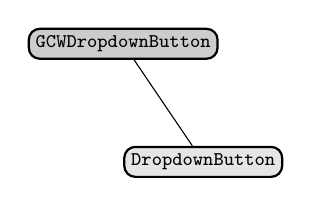
\begin{tikzpicture}
    \node [root] {GCWDropdownButton}
    child { node [selected] {DropdownButton}
        edge from parent [-]
    };
\end{tikzpicture}
\captionof{figure}{GCWDropdownButton}
\label{fig: GCWDropdownButton}
\begin{table}[H]
\begin{tabular}[h]{p{2cm}p{9cm}}
    \caption{GCWDropdownButton}
    Aim       & shows a Dropdown-List\\
    Import    & GCWizard/lib/widgets/common/base/gcw\_dropdownbutton.dart\\
    Parameter & items\newline
                value\newline
                Function onChanged\\
    \label{tab:GCWDropdownButton}
\end{tabular}
\end{table}
\paragraph*{Example} \,
\begin{lstlisting}
Widget build(BuildContext context) {
    return Column(
        children: <Widget>[
        ...
        ],
    );
}
\end{lstlisting}
\captionof{lstlisting}{Example GCWDropdownButton}
\label{fig: ExampleGCWDropdownButton}

\newpage
\section{Numeral input}
\subsection{GCWDoubleSpinner}
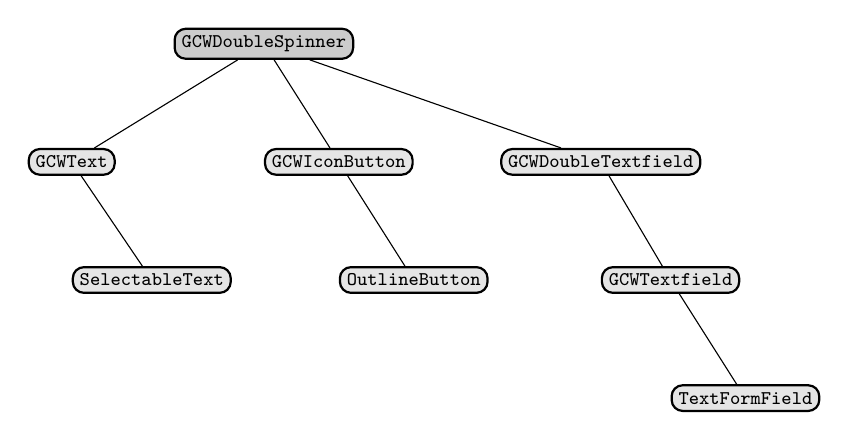
\begin{tikzpicture}
    \node [root] {GCWDoubleSpinner}
    child { node [selected] {GCWText}
        child { node [selected] {SelectableText}
        }
    }
    child [missing]
    child { node [selected] {GCWIconButton}
        edge from parent [-]
        child { node [selected] {OutlineButton}
        }
    }
    child [missing]
    child { node [selected] {GCWDoubleTextfield}
        child { node [selected] {GCWTextfield}
            child { node [selected] {TextFormField}
                edge from parent [-]
            }
        }
    };
\end{tikzpicture}
\captionof{figure}{GCWDoubleSpinner}
\label{fig: GCWDoubleSpinner}
\begin{table}[H]
\begin{tabular}[h]{p{2cm}p{9cm}}
    \caption{GCWDoubleSpinner}
    Aim       & Provides a spinner to enter a double value\\
    Import    & GCWizard/lib/widgets/common/gcw\_double\_spinner.dart\\
    Parameter & TextEditingController controller\newline
                Function onChanged\newline
                title\newline
                value\newline
                min\newline
                max\newline
                numberDecimalDigits\newline
                SpinnerLayout layout\newline
                FocusNode focusNode\\
    \label{tab:GCWDoubleSpinner}
\end{tabular}
\end{table}
\paragraph*{Example} \,
\begin{lstlisting}
Widget build(BuildContext context) {
    return Column(
        children: <Widget>[
        ...
        ],
    );
}
\end{lstlisting}
\captionof{lstlisting}{Example GCWDoubleSpinner}
\label{fig: ExampleGCWDoubleSpinner}

\newpage
\subsection{GCWDoubleTextfield}
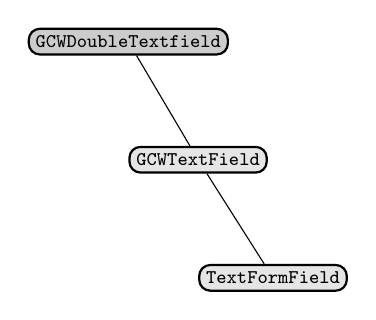
\begin{tikzpicture}
    \node [root] {GCWDoubleTextfield}
    child { node [selected] {GCWTextField}
        edge from parent [-]
        child { node [selected] {TextFormField}
            edge from parent [-]
        };
    };
\end{tikzpicture}
\captionof{figure}{GCWDoubleTextfield}
\label{fig: GCWDoubleTextfield}
\begin{table}[H]
\begin{tabular}[h]{p{2cm}p{9cm}}
    \caption{GCWDoubleTextfield}
    Aim       & Provides a Textfiled, which only accepts double-Numbers\\
    Import    & GCWizard/lib/widgets/common/gcw\_double\_textfield.dart\\
    Parameter & TextEditingController controller\newline
                Function onChanged\newline
                List<TextInputFormatter> inputFormatters\newline
                TextInputType keyboardType\newline
                hintText\newline
                min\newline
                max\newline
                FocusNode focusNode\newline
                numberDecimalDigits\newline\\
    \label{tab:GCWDoubleTextfield}
\end{tabular}
\end{table}
\paragraph*{Example} \,
\begin{lstlisting}
Widget build(BuildContext context) {
    return Column(
        children: <Widget>[
            ...
            Inhalt...
        ],
    );
}
\end{lstlisting}
\captionof{lstlisting}{Example GCWDoubleTextfield}
\label{fig: ExampleGCWDoubleTextfield}

\newpage
\subsection{GCWIntegerListTextfield}
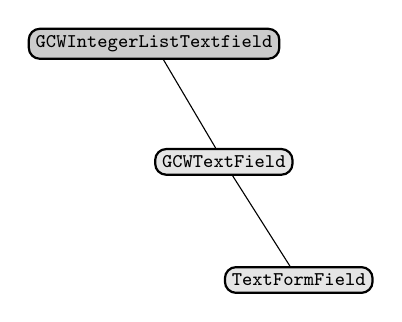
\begin{tikzpicture}
    \node [root] {GCWIntegerListTextfield}
    child { node [selected] {GCWTextField}
        edge from parent [-]
        child { node [selected] {TextFormField}
            edge from parent [-]
        };
    };
\end{tikzpicture}
\captionof{figure}{GCWIntegerListTextfield}
\label{fig: GCWIntegerListTextfield}
\begin{table}[H]
\begin{tabular}[h]{p{2cm}p{9cm}}
    \caption{GCWIntegerListTextfield}
    Aim       & Reads a list of integers\\
    Import    & GCWizard/lib/widgets/common/gcw\_integer\_list\_textfield.dart\\
    Parameter & TextEditingController controller\newline
                Function onChanged\newline
                hintText\\
    \label{tab:GCWIntegerListTextfield}
\end{tabular}
\end{table}
\paragraph*{Example} \,
\begin{lstlisting}
Widget build(BuildContext context) {
    return Column(
        children: <Widget>[
            ...
            Inhalt...
        ],
    );
}
\end{lstlisting}
\captionof{lstlisting}{Example GCWIntegerListTextfield}
\label{fig: ExampleGCWIntegerListTextfield}

\newpage
\subsection{GCWIntegerSpinner}
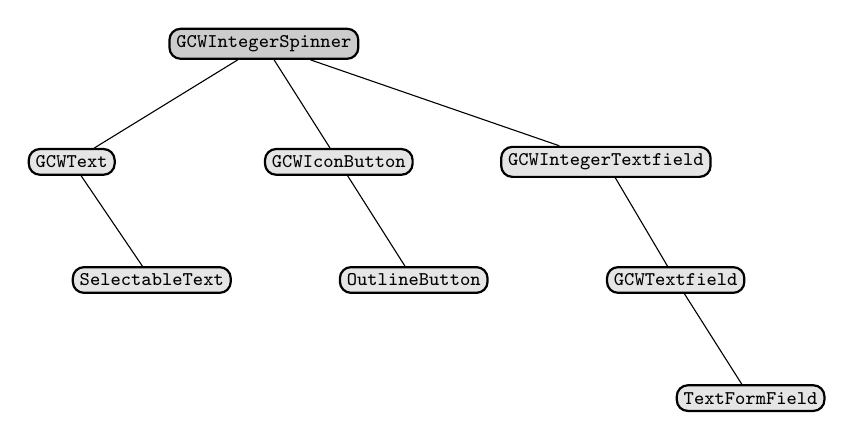
\begin{tikzpicture}
    \node [root] {GCWIntegerSpinner}
    child { node [selected] {GCWText}
        child { node [selected] {SelectableText}
        }
    }
    child [missing]
    child { node [selected] {GCWIconButton}
        edge from parent [-]
        child { node [selected] {OutlineButton}
        }
    }
    child [missing]
    child { node [selected] {GCWIntegerTextfield}
        child { node [selected] {GCWTextfield}
            child { node [selected] {TextFormField}
                edge from parent [-]
            }
        }
    };
\end{tikzpicture}
\captionof{figure}{GCWIntegerSpinner}
\label{fig: GCWIntegerSpinner}
\begin{table}[H]
\begin{tabular}[h]{p{2cm}p{9cm}}
    \caption{GCWIntegerSpinner}
    Aim       & Provides a spinner to enter an integer value\\
    Import    & GCWizard/lib/widgets/common/gcw\_integer\_spinner.dart\\
    Parameter & Function onChanged\newline
                title\newline
                value\newline
                min\newline
                max\newline
                controller\newline
                SpinnerLayout layout\newline
                focusNode\\
    \label{tab:GCWIntegerSpinner}
\end{tabular}
\end{table}
\paragraph*{Example} \,
\begin{figure}[H]
    \centering
    
\includegraphics[height=0.75cm]{Bilder/SpinnerInput}
    \caption[]{Example GCWIntegerSpinner}
    \label{fig:GCWIntegerSpinner}
\end{figure}
\begin{lstlisting}
Widget build(BuildContext context) {
    return Column(
        children: <Widget>[
...
            GCWIntegerSpinner(
                title: i18n(context, 'affine_key_b'),
                min: 0,
                max: 25,
                value: _currentKeyBIndex,
                onChanged: (value) {
                    setState(() {
                        _currentKeyBIndex = value;
                    });
                },
            ),
...
        ],
    );
}
\end{lstlisting}
\captionof{lstlisting}{Example GCWIntegerSpinner}
\label{fig: ExampleGCWIntegerSpinner}

\newpage
\subsection{GCWIntegerTextfield}
\begin{table}[H]
\begin{tabular}[h]{p{2cm}p{9cm}}
    \caption{GCWIntegerTextfield}
    Aim       & \\
    Import    & \\
    Parameter & \\
    \label{tab:GCWIntegerTextfield}
\end{tabular}
\end{table}
\paragraph*{Example} \,
\begin{lstlisting}
Widget build(BuildContext context) {
    return Column(
        children: <Widget>[
            ...
            Inhalt...
        ],
    );
}
\end{lstlisting}
\captionof{lstlisting}{Example GCWIntegerTextfield}
\label{fig: ExampleGCWIntegerTextfield}

\newpage
\subsection{GCWNumeralBaseSpinner}
\begin{table}[H]
\begin{tabular}[h]{p{2cm}p{9cm}}
    \caption{GCWNumeralBaseSpinner}
    Aim       & \\
    Import    & \\
    Parameter & \\
    \label{tab:GCWNumeralBaseSpinner}
\end{tabular}
\end{table}
\paragraph*{Example} \,
\begin{lstlisting}
Widget build(BuildContext context) {
    return Column(
        children: <Widget>[
            ...
            Inhalt...
        ],
    );
}
\end{lstlisting}
\captionof{lstlisting}{Example GCWNumeralBaseSpinner}
\label{fig: ExampleGCWNumeralBaseSpinner}

\newpage
\section{Unit-Inputs}
\subsection{GCWUnitDropdownButton}
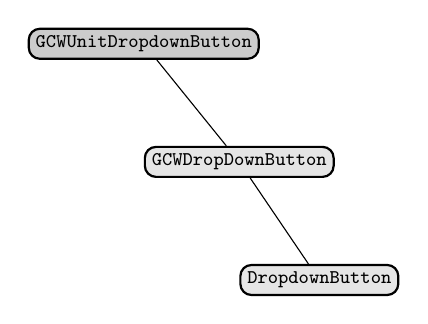
\begin{tikzpicture}
    \node [root] {GCWUnitDropdownButton}
    child { node [selected] {GCWDropDownButton}
        child { node [selected] {DropdownButton}
        }
    };
\end{tikzpicture}
\captionof{figure}{GCWUnitDropdownButton}
\label{fig: GCWUnitDropdownButton}
\begin{table}[H]
\begin{tabular}[h]{p{2cm}p{9cm}}
    \caption{GCWUnitDropdownButton}
    Aim       & Shows a Dropdown to enter units.\\
    Import    & GCWizard/lib/widgets/common/units/gcw\_unit\_dropdownbutton.dart\\
    Parameter & Function onChanged\newline
                Unit value\newline
                List<Unit> unitList\newline
                UnitCategory unitCategory\newline
                bool onlyShowSymbols\\
    \label{tab:GCWUnitDropdownButton}
\end{tabular}
\end{table}
\paragraph*{Example} \,
\begin{lstlisting}
Widget build(BuildContext context) {
    return Column(
        children: <Widget>[
            ...
            Inhalt...
        ],
    );
}
\end{lstlisting}
\captionof{lstlisting}{Example GCWUnitDropdownButton}
\label{fig: ExampleGCWUnitDropdownButton}

\newpage
\subsection{GCWUnitInput}
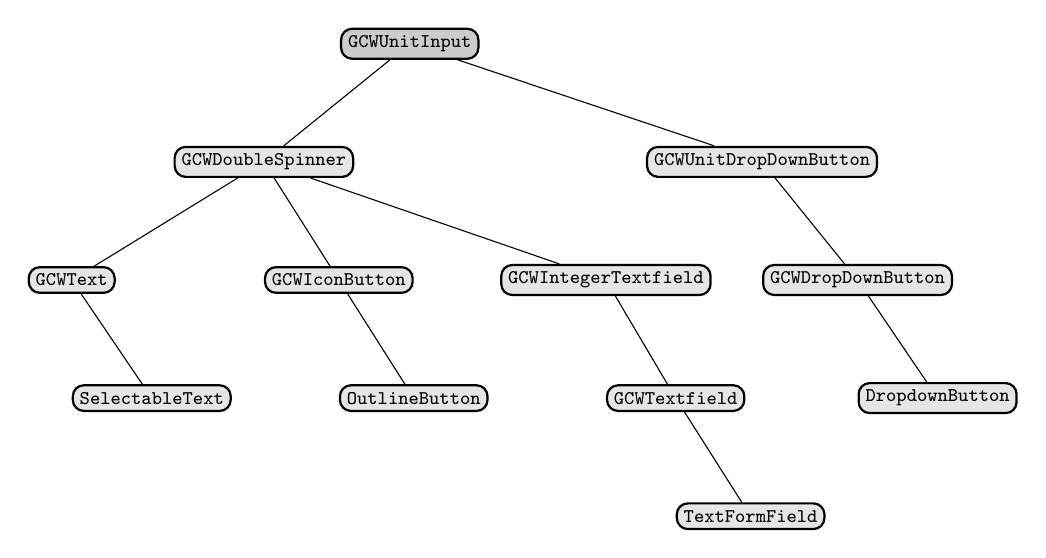
\begin{tikzpicture}
    \node [root] {GCWUnitInput}
    child { node [selected] {GCWDoubleSpinner}
        child { node [selected] {GCWText}
            child { node [selected] {SelectableText}
            }
        }
        child [missing]
        child { node [selected] {GCWIconButton}
            edge from parent [-]
            child { node [selected] {OutlineButton}
            }
        }
        child [missing]
        child { node [selected] {GCWIntegerTextfield}
            child { node [selected] {GCWTextfield}
                child { node [selected] {TextFormField}
                    edge from parent [-]
                }
            }
        }
    }
    child [missing]
    child [missing]
    child [missing]
    child { node [selected] {GCWUnitDropDownButton}
        child { node [selected] {GCWDropDownButton}
            child { node [selected] {DropdownButton}
            }
        }
    };
\end{tikzpicture}
\captionof{figure}{GCWUnitInput}
\label{fig: GCWUnitInput}
\begin{table}[H]
\begin{tabular}[h]{p{2cm}p{9cm}}
    \caption{GCWUnitInput}
    Aim       & Shows a dropdown and a doubleSpinner to enter an unit with value.\\
    Import    & GCWizard/lib/widgets/common/units/gcw\_unit\_input.dart\\
    Parameter & min\newline
                numberDecimalDigits\newline
                double value\newline
                List<Unit> unitList\newline
                UnitCategory unitCategory\newline
                title\\
    \label{tab:GCWUnitInput}
\end{tabular}
\end{table}
\paragraph*{Example} \,
\begin{lstlisting}
Widget build(BuildContext context) {
    return Column(
        children: <Widget>[
            ...
            GCWUnitInput(
                value: _currentInputMass,
                title: i18n(context, 'projectiles_mass'),
                unitList: allMasses(),
                onChanged: (value) {
                    setState(() {
                        _currentInputMass = value;
                    });
                },
             )
             ...
        ],
    );
}
\end{lstlisting}
\captionof{lstlisting}{Example GCWUnitInput}
\label{fig: ExampleGCWUnitInput}

\newpage
\subsection{GCWUnitPrefixDropdownButton}
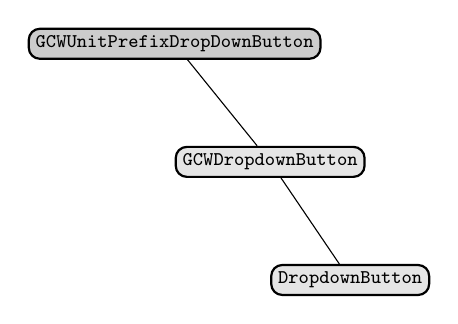
\begin{tikzpicture}
    \node [root] {GCWUnitPrefixDropDownButton}
    child { node [selected] {GCWDropdownButton}
        child { node [selected] {DropdownButton}
        }
    };
\end{tikzpicture}
\captionof{figure}{GCWUnitPrefixDropdownButton}
\label{fig: GCWUnitPrefixDropdownButton}
\begin{table}[H]
\begin{tabular}[h]{p{2cm}p{9cm}}
    \caption{GCWUnitPrefixDropdownButton}
    Aim       & Shows a dropdown to enter prefixes for units\\
    Import    & GCWizard/lib/widgets/common/units/gcw\_unit\_prefix\_dropdownbutton.dart\\
    Parameter & Function onChanged\newline
                UnitPrefix value\newline
                bool onlyShowSymbols\\
    \label{tab:GCWUnitPrefixDropdownButton}
\end{tabular}
\end{table}
\paragraph*{Example} \,
\begin{lstlisting}
Widget build(BuildContext context) {
    return Column(
        children: <Widget>[
            ...
            Inhalt...
        ],
    );
}
\end{lstlisting}
\captionof{lstlisting}{Example GCWUnitPrefixDropdownButton}
\label{fig: ExampleGCWUnitPrefixDropdownButton}

\newpage
\subsection{GCWUnits}
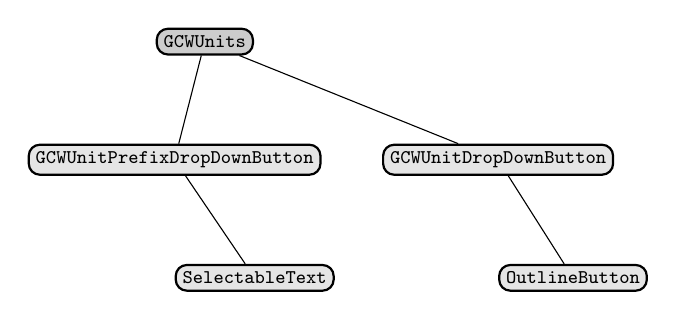
\begin{tikzpicture}
    \node [root] {GCWUnits}
    child { node [selected] {GCWUnitPrefixDropDownButton}
        child { node [selected] {SelectableText}
        }
    }
    child [missing]
    child [missing]
    child { node [selected] {GCWUnitDropDownButton}
        edge from parent [-]
        child { node [selected] {OutlineButton}
        }
    };
\end{tikzpicture}
\captionof{figure}{GCWUnits}
\label{fig: GCWUnits}
\begin{table}[H]
    \begin{tabular}[h]{p{2cm}p{9cm}}
        \caption{GCWUnits}
        Aim       & Shows a dropdown to enter prefixes and also a dropwdown to enter units\\
        Import    & GCWizard/lib/widgets/common/units/gcw\_units.dart\\
        Parameter & UnitCategory unitCategory\newline
                    Function onChanged\newline
                    bool onlyShowUnitSymbols\newline
                    bool onlyShowPrefixSymbols\newline
                    Map<String, dynamic> value\\
        \label{tab:GCWUnits}
    \end{tabular}
\end{table}
\paragraph*{Example} \,
\begin{lstlisting}
    Widget build(BuildContext context) {
        return Column(
            children: <Widget>[
                ...
                GCWUnits(
                    value: _currentOutputUnit,
                    unitCategory: _currentMode,
                    onlyShowPrefixSymbols: false,
                    onChanged: (value) {
                        setState(() {
                            _currentOutputUnit = value;
                        });
                    },
                ),
                ...
            ],
        );
    }
\end{lstlisting}
\captionof{lstlisting}{Example GCWUnits}
\label{fig: ExampleGCWUnits}

\newpage
\section{Miscellaneous inputs}
\subsection{GCWABCDropdownButton}
\begin{table}[H]
\begin{tabular}[h]{p{2cm}p{9cm}}
    \caption{GCWABCDropdownButton}
    Aim       & \\
    Import    & \\
    Parameter & \\
    \label{tab:GCWABCDropdownButton}
\end{tabular}
\end{table}
\paragraph*{Example} \,
\begin{lstlisting}
Widget build(BuildContext context) {
    return Column(
        children: <Widget>[
            ...
            Inhalt...
        ],
    );
}
\end{lstlisting}
\captionof{lstlisting}{Example GCWABCDropdownButton}
\label{fig: ExampleGCWABCDropdownButton}

\newpage
\subsection{GCWDropdownSpinner}
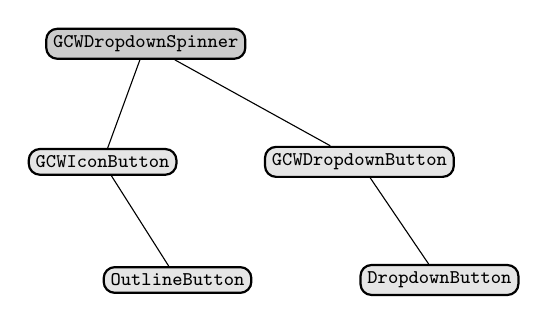
\begin{tikzpicture}
    \node [root] {GCWDropdownSpinner}
    child { node [selected] {GCWIconButton}
        child { node [selected] {OutlineButton}
        }
    }
    child [missing]
    child { node [selected] {GCWDropdownButton}
        edge from parent [-]
        child { node [selected] {DropdownButton}
        }
    };
\end{tikzpicture}
\captionof{figure}{GCWDropdownSpinner}
\label{fig: GCWDropdownSpinner}
\begin{table}[H]
\begin{tabular}[h]{p{2cm}p{9cm}}
    \caption{GCWDialog}
    Aim       & \\
    Import    & GCWizard/lib/widgets/common/gcw\_dropdown\_spinner.dart\\
    Parameter & Function onChanged;
                index;
                List<dynamic> items;
                SpinnerLayout layout;
                String title;\\
    \label{tab:GCWDropdownSpinner}
\end{tabular}
\end{table}
\paragraph*{Example} \,
\begin{lstlisting}
Widget build(BuildContext context) {
    return Column(
        children: <Widget>[
            ...
            GCWDropDownSpinner(
                title: i18n(context, 'affine_key_a'),
                index: _currentKeyAIndex,
                items: aKeys.map((item) => GCWText(text: item.toString())).toList(),
                onChanged: (value) {
                    setState(() {
                        _currentKeyAIndex = value;
                    });
                },
            ),
            ...
        ],
    );
}
\end{lstlisting}
\captionof{lstlisting}{Example GCWDropdownSpinner}
\label{fig: ExampleGCWDropdownSpinner}

\newpage
\subsection{GCWDatePicker}
\begin{table}[H]
\begin{tabular}[h]{p{2cm}p{9cm}}
    \caption{GCWDatePicker}
    Aim       & \\
    Import    & \\
    Parameter & \\
    Example   & \\
    \label{tab:GCWDatePicker}
\end{tabular}
\end{table}

\newpage
\subsection{GCWDateTimePicker}
\begin{table}[H]
\begin{tabular}[h]{p{2cm}p{9cm}}
    \caption{GCWDateTimePicker}
    Aim       & \\
    Import    & \\
    Parameter & \\
    \label{tab:GCWDateTimePicker}
\end{tabular}
\end{table}
\paragraph*{Example} \,
\begin{lstlisting}
Widget build(BuildContext context) {
    return Column(
        children: <Widget>[
            ...
            Inhalt...
        ],
    );
}
\end{lstlisting}
\captionof{lstlisting}{Example GCWDateTimePicker}
\label{fig: ExampleGCWDateTimePicker}

\newpage
\section{Buttons}
\subsection{GCWButton}
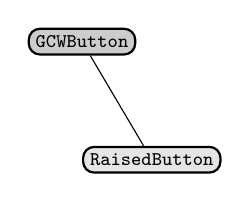
\begin{tikzpicture}
    \node [root] {GCWButton}
        child { node [selected] {RaisedButton}
        };
\end{tikzpicture}
\captionof{figure}{GCWButton}
\label{fig: GCWButton}
\begin{table}[H]
\begin{tabular}[h]{p{2cm}p{9cm}}
    \caption{GCWButton}
    Aim       & \\
    Import    & \\
    Parameter & \\
    Example   & \\
    \label{tab:GCWButton}
\end{tabular}
\end{table}

\newpage
\subsection{GCWIconButton}
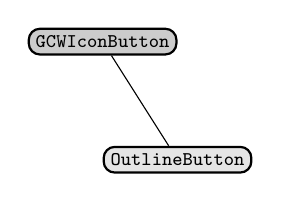
\begin{tikzpicture}
    \node [root] {GCWIconButton}
    child { node [selected] {OutlineButton}
    };
\end{tikzpicture}
\captionof{figure}{GWCIconButton}
\label{fig: GWCIconButton}
\begin{table}[H]
\begin{tabular}[h]{p{2cm}p{9cm}}
    \caption{GCWIconButton}
    Aim       & \\
    Import    & \\
    Parameter & \\
    \label{tab:GCWIconButton}
\end{tabular}
\end{table}
\paragraph*{Example} \,
\begin{lstlisting}
Widget build(BuildContext context) {
    return Column(
        children: <Widget>[
            ...
            Inhalt...
        ],
    );
}
\end{lstlisting}
\captionof{lstlisting}{Example GCWIconButton}
\label{fig: ExampleGCWIconButton}

\newpage
\subsection{GCWEncryptButtonBar}
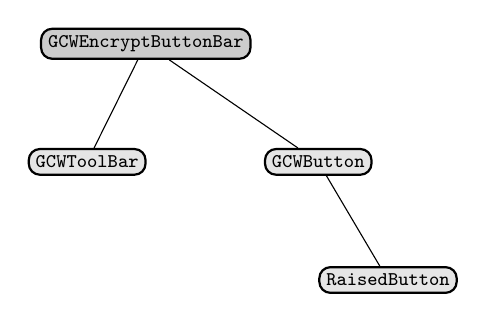
\begin{tikzpicture}
    \node [root] {GCWEncryptButtonBar}
    child { node [selected] {GCWToolBar}
    }
    child [missing]
    child { node [selected] {GCWButton}
        edge from parent [-]
        child { node [selected] {RaisedButton}
        }
    };
\end{tikzpicture}
\captionof{figure}{GCWEncryptButtonBar}
\label{fig: GCWEncryptButtonBar}
\begin{table}[H]
\begin{tabular}[h]{p{2cm}p{9cm}}
    \caption{GCWEncryptButtonBar}
    Aim       & Displays a Button Bar with two buttons: Encode, Decode\\
    Import    & GCWizard/lib/widgets/common/gcw\_encrypt\_buttonbar.dart\\
    Parameter & Function onPressedEncode\newline
                Function onPressedDecode\\
    \label{tab:GCWEncryptButtonBar}
\end{tabular}
\end{table}
\paragraph*{Example} \,
\begin{lstlisting}
Widget build(BuildContext context) {
    return Column(
        children: <Widget>[
            ...
            Inhalt...
        ],
    );
}
\end{lstlisting}
\captionof{lstlisting}{Example GCWEncryptButtonBar}
\label{fig: ExampleGCWEncryptButtonBar}

\newpage
\subsection{GCWToolBar}
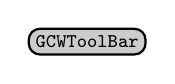
\begin{tikzpicture}
    \node [root] {GCWToolBar};
\end{tikzpicture}
\captionof{figure}{GCWToolBar}
\label{fig: GCWToolBar}
\begin{table}[H]
\begin{tabular}[h]{p{2cm}p{9cm}}
    \caption{GCWToolBar}
    Aim       & Displays a Button Bar\\
    Import    & GCWizard/lib/widgets/common/gcw\_buttonbar.dart\\
    Parameter & List<widget> children\\
    \label{tab:GCWToolBar}
\end{tabular}
\end{table}
\paragraph*{Example} \,
\begin{lstlisting}
Widget build(BuildContext context) {
    return Column(
        children: <Widget>[
            ...
            Inhalt...
        ],
    );
}
\end{lstlisting}
\captionof{lstlisting}{Example GCWToolBar}
\label{fig: ExampleGCWToolBar}

\newpage
\section{Switches}
\subsection{GCWSwitch}
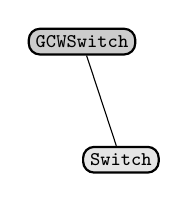
\begin{tikzpicture}
    \node [root] {GCWSwitch}
    child { node [selected] {Switch}
    };
\end{tikzpicture}
\captionof{figure}{GCWSwitch}
\label{fig: GCWSwitch}
\begin{table}[H]
\begin{tabular}[h]{p{2cm}p{9cm}}
    \caption{GCWSwitch}
    Aim       & \\
    Import    & GCWizard/lib/widgets/common/base/gcw\_switch.dart\\
    Parameter & String text\newline
                Function onChanged\newline
                value\newline
                inactiveTrackColor\newline
                inactiveThumbColor\newline
                activeThumbColor\newline
                activeTrackColor\\
    \label{tab:GCWSwitch}
\end{tabular}
\end{table}
\paragraph*{Example} \,
\begin{lstlisting}
    Inhalt...
        ],
    );
}
\end{lstlisting}
\captionof{lstlisting}{Example GCWSwitch}
\label{fig: ExampleGCWSwitch}

\newpage
\subsection{GCWOnOffSwitch}
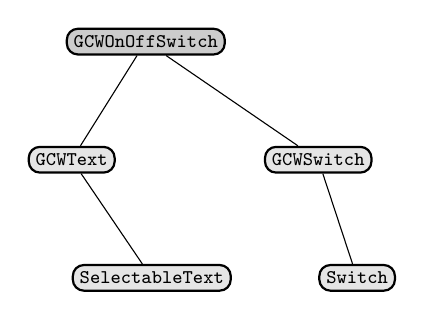
\begin{tikzpicture}
    \node [root] {GCWOnOffSwitch}
    child { node [selected] {GCWText}
        child { node [selected] {SelectableText}
        }
    }
    child [missing]
    child { node [selected] {GCWSwitch}
        child { node [selected] {Switch}
        }
    };
\end{tikzpicture}
\captionof{figure}{GCWOnOffSwitch}
\label{fig: GCWOnOffSwitch}
\begin{table}[H]
\begin{tabular}[h]{p{2cm}p{9cm}}
    \caption{GCWOnOffSwitch}
    Aim       & Sets an option to ON or OFF\\
    Import    & GCWizard/lib/widgets/common/gcw\_onoff\_switch.dart\\
    Parameter & Function onChanged;
                String title;
                value;
                bool notitle;\\
    \label{tab:GCWOnOffSwitch}
\end{tabular}
\end{table}
\paragraph*{Example} \,
\begin{lstlisting}
    Inhalt...
        ],
    );
}
\end{lstlisting}
\captionof{lstlisting}{Example GCWOnOffSwitch}
\label{fig: ExampleGCWOnOffSwitch}

\newpage
\subsection{GCWTwoOptionsSwitch}
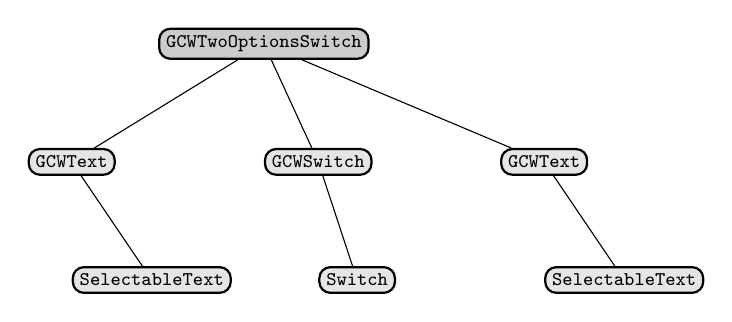
\begin{tikzpicture}
    \node [root] {GCWTwoOptionsSwitch}
    child { node [selected] {GCWText}
        child { node [selected] {SelectableText}
        }
    }
    child [missing]
    child { node [selected] {GCWSwitch}
        child { node [selected] {Switch}
        }
    }
    child [missing]
    child { node [selected] {GCWText}
        child { node [selected] {SelectableText}
        }
    };
\end{tikzpicture}
\captionof{figure}{GCWTwoOptionsSwitch}
\label{fig: GCWTwoOptionsSwitch}
\begin{table}[H]
    \begin{tabular}[h]{p{2cm}p{9cm}}
        \caption{GCWTwoOptionsSwitch}
        Aim       & Switches between two options and returns GCWSwitchPosition.left or GCWSwitchPosition.right\\
        Import    & GCWizard/lib/widgets/common/gcw\_twooptions\_switch.dart\\
        Parameter & String title\newline
                    Function onChanged\newline
                    String leftvalue\newline
                    String rightvalue\newline
                    GCWSwitchPosition value\newline
                    bool alternativeColor\\
        \label{tab:GCWTwoOptionsSwitch}
\end{tabular}
\end{table}
\paragraph{Example} \,
\begin{figure}[H]
    \centering
    
\includegraphics[height=0.75cm]{Bilder/SwitchTwoOptions}
    \caption[]{Example GCWTwoOptionsSwitch}
    \label{fig:switchtwooptions}
\end{figure}
\begin{lstlisting}
...
_currentMode == GCWSwitchPosition.left
...
GCWTwoOptionsSwitch(
    title = i18n(context, 'common_mode');
    leftvalue = i18n(context, 'common_encrypt');
    rightvalue = i18n(context, 'common_decrypt');
    value = _currentmode;
    onChanged: (value) {
        setState(() {
            _currentMode = value;
        });
    },
),
...
\\within the creation of a widget
_currentMode == GCWSwitchPosition.left
? ...
: ...,
...
\\ within a method:
if (_currentMode == GCWSwitchPosition.left) {
    ...
} else {
    ...
}
...
        ],
    );
}
\end{lstlisting}
\captionof{lstlisting}{Example GCWSwitchPosition}
\label{fig: ExampleGCWSwitchPosition}

\newpage
\section{Output}
\subsection{GCWText}
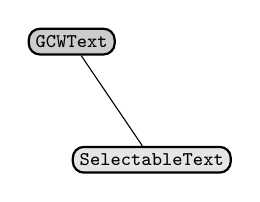
\begin{tikzpicture}
    \node [root] {GCWText}
    child { node [selected] {SelectableText}
    };
\end{tikzpicture}
\captionof{figure}{GCWText}
\label{fig: GCWText}
\begin{table}[H]
\begin{tabular}[h]{p{2cm}p{9cm}}
    \caption{GCWText}
    Aim       & Print text\\
    Import    & GCWizard/lib/widgets/common/base/gcw\_text.dart\\
    Parameter & String text\newline
                Alignment align\newline
                TextAlign textAlign\newline
                TextStyle style\\
    \label{tab:GCWText}
\end{tabular}
\end{table}
\paragraph*{Example} \,
\begin{lstlisting}
    Inhalt...
\end{lstlisting}
\captionof{lstlisting}{Example GCWIntegerSpinner}
\label{fig: ExampleGCWIntegerSpinner}

\newpage
\subsection{GCWOutputText}
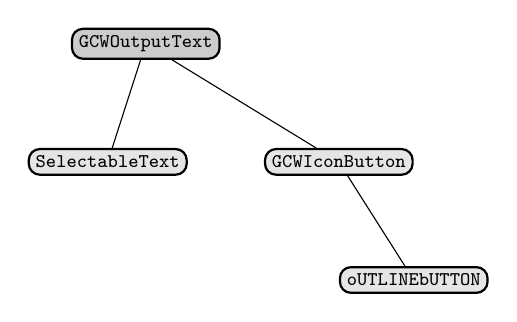
\begin{tikzpicture}
    \node [root] {GCWOutputText}
    child { node [selected] {SelectableText}
    }
    child [missing]
    child { node [selected] {GCWIconButton}
        child { node [selected] {oUTLINEbUTTON}
        }
    };
\end{tikzpicture}
\captionof{figure}{GCWOutputText}
\label{fig: GCWOutputText}
\begin{table}[H]
    \begin{tabular}[h]{p{2cm}p{9cm}}
        \caption{GCWOutput}
        Aim       & Print text and provide a copyToClipboard-Button\\
        Import    & GCWizard/lib/widgets/common/base/gcw\_output\_text.dart\\
        Parameter & String text\newline
                    Alignment align\newline
                    bool isMonotype\newline
                    TextStyle style\newline
                    bool suppressCopyButton\newline
                    String copyText\\
        \label{tab:GCWOutputText}
    \end{tabular}
\end{table}
\paragraph*{Example} \,
\begin{lstlisting}
    Inhalt...
        ],
    );
}
\end{lstlisting}
\captionof{lstlisting}{Example GCWOutputText}
\label{fig: ExampleGCWOutputText}

\newpage
\subsection{GCWOutput}
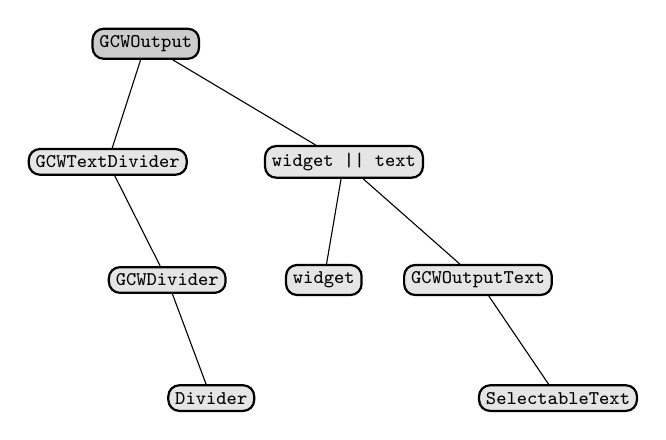
\begin{tikzpicture}
    \node [root] {GCWOutput}
    child { node [selected] {GCWTextDivider}
        child { node [selected] {GCWDivider}
            child { node [selected] {Divider}
            }
        }
    }
    child [missing]
    child { node [selected] {widget || text}
        child { node [selected] {widget}
        }
        child { node [selected] {GCWOutputText}
            child { node [selected] {SelectableText}
            }
        }
    };
\end{tikzpicture}
\captionof{figure}{GCWOutput}
\label{fig: GCWOutput}
\begin{table}[H]
\begin{tabular}[h]{p{2cm}p{9cm}}
    \caption{GCWOutput}
    Aim       & Print a title and a childe -- widget or text\\
    Import    & GCWizard/lib/widgets/common/gcw\_output.dart\\
    Parameter & dynamic child\newline
                String title\\
    \label{tab:GCWOutput}
\end{tabular}
\end{table}
\paragraph*{Example} \,
\begin{lstlisting}
    ...
GCWOutput(
    text: output,
),
...
        ],
    );
}
\end{lstlisting}
\captionof{lstlisting}{Example GCWOutput}
\label{fig: ExampleGCWOutput}

\newpage
\subsection{GCWDefaultOutput}
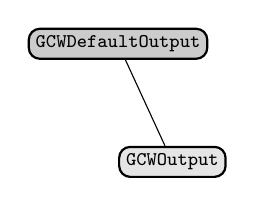
\begin{tikzpicture}
    \node [root] {GCWDefaultOutput}
    child { node [selected] {GCWOutput}
    };
\end{tikzpicture}
\captionof{figure}{GCWDefaultOutput}
\label{fig: GCWDefaultOutput}
\begin{table}[H]
\begin{tabular}[h]{p{2cm}p{9cm}}
    \caption{GCWDefaultOutput}
    Aim       & Print the default-Output-Text and a widget\\
    Import    & GCWizard/lib/widgets/common/gcw\_default\_output.dart\\
    Parameter & dynamic child\\
    \label{tab:GCWDefaultOutput}
\end{tabular}
\end{table}
\paragraph*{Example} \,
\begin{lstlisting}
    Inhalt...
\end{lstlisting}
\captionof{lstlisting}{Example GCWDefaultOutput}
\label{fig: ExampleGCWDefaultOutput}

\newpage
\subsection{GCWMultipleOutput}
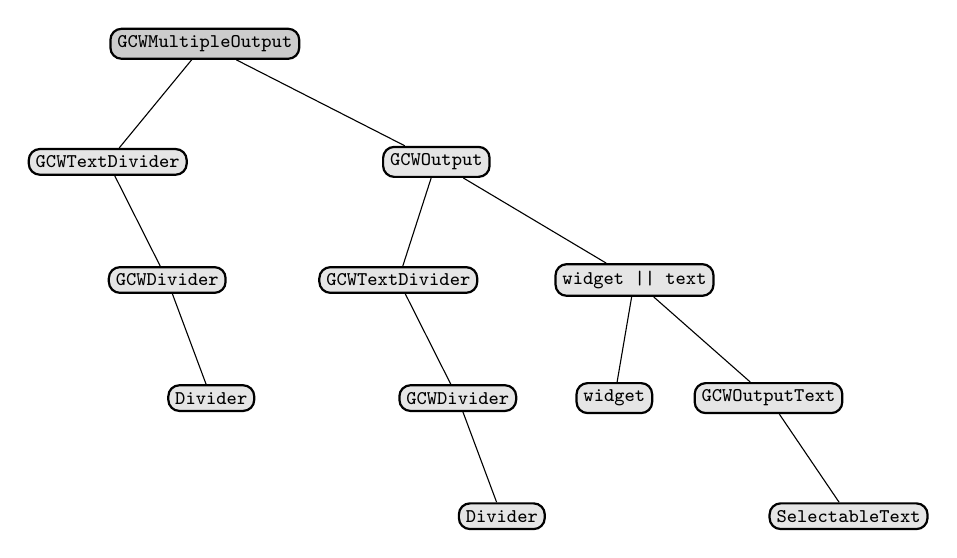
\begin{tikzpicture}
    \node [root] {GCWMultipleOutput}
    child { node [selected] {GCWTextDivider}
        child { node [selected] {GCWDivider}
            child { node [selected] {Divider}
            }
        }
    }
    child [missing]
    child [missing]
    child { node [selected] {GCWOutput}
        child { node [selected] {GCWTextDivider}
            child { node [selected] {GCWDivider}
                child { node [selected] {Divider}
                }
            }
        }
        child [missing]
        child { node [selected] {widget || text}
            child { node [selected] {widget}
            }
            child { node [selected] {GCWOutputText}
                child { node [selected] {SelectableText}
                }
            }
        }
    };
\end{tikzpicture}
\captionof{figure}{GCWMultipleOutput}
\label{fig: GCWMultipleOutput}
\begin{table}[H]
\begin{tabular}[h]{p{2cm}p{9cm}}
    \caption{GCWMultipleOutput}
    Aim       & Print multiple lines of output\\
    Import    & GCWizard/lib/widgets/common/gcw\_multiple\_output.dart\\
    Parameter & List<dynamic> children\newline
                bool suppressDefaultTitle\\
    \label{tab:GCWMultipleOutput}
\end{tabular}
\end{table}
\paragraph*{Example} \,
\begin{lstlisting}
    Inhalt...
        ],
    );
}
\end{lstlisting}
\captionof{lstlisting}{Example GCWMultipleOutput}
\label{fig: ExampleGCWMultipleOutput}

\newpage
\section{Messages}
\subsection{GCWToast}
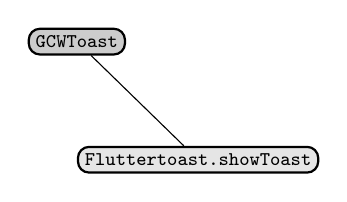
\begin{tikzpicture}
    \node [root] {GCWToast}
    child { node [selected] {Fluttertoast.showToast}
    };
\end{tikzpicture}
\captionof{figure}{GCWToast}
\label{fig: GCWToast}
\begin{table}[H]
\begin{tabular}[h]{p{2cm}p{9cm}}
    \caption{GCWToast}
    Aim       & Shows a small message that pops up at the bottom of the device screen and immediately disappears on it’s own after a delay of few seconds.\\
    Import    & package:gc\_wizard/widgets/common/base/gcw\_toast.dart\\
    Parameter & String text \\
    \label{tab:GCWToast}
\end{tabular}
\end{table}
\paragraph*{Example} \,
\begin{lstlisting}
    Inhalt...
        ],
    );
}
\end{lstlisting}
\captionof{lstlisting}{Example GCWToast}
\label{fig: ExampleGCWToastr}

\newpage
\subsection{GCWDialog}
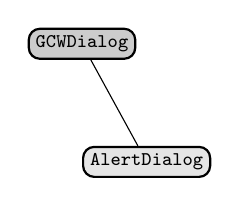
\begin{tikzpicture}
    \node [root] {GCWDialog}
    child { node [selected] {AlertDialog}
    };
\end{tikzpicture}
\captionof{figure}{GCWDialog}
\label{fig: GCWDialog}
\begin{table}[H]
\begin{tabular}{p{2cm}p{9cm}}
    \caption{GCWDialog}
    Aim         & Informs the user about situations that require acknowledgement. A dialog has an optional title and an optional list of actions. The title is displayed above the content and the actions are displayed below the content.\\
    Import      & package:gc\_wizard/widgets/common/base/gcw\_dialog.dart\\
    Parameter   & String title\newline
                  content\newline
                  actions\\
    \label{tab:GCWDialog}
\end{tabular}
\end{table}
\paragraph*{Example} \,
\begin{lstlisting}
    Inhalt...
            ],
    );
}

\end{lstlisting}
\captionof{lstlisting}{Example GCWDialog}
\label{fig: ExampleGCWDialogr}
